\documentclass[14pt]{beamer}
\usetheme{zdr}
%
\usepackage{booktabs} % \toprule, etc
% My macros
/Users/zach/Git/zachs_macros/zachs_macros.tex

% Custom colors
\usepackage{color}
\definecolor{ao}{rgb}{0.0, 0.5, 0.0}
\setbeamercolor{alerted text}{fg=palered}

% Configure fonts
\usefonttheme{professionalfonts}
\usefonttheme{serif}
\usepackage{fontspec}
\setmainfont{Helvetica Neue}
\setbeamerfont{note page}{family*=pplx,size=\footnotesize} % Palatino for notes

% Configure listings for R
\usepackage{listings}

\lstset{frame=tb,
language=R,
keywordstyle=\color{blue},
otherkeywords={!,!=,~,$,*,\&,\%/\%,\%*\%,\%\%,<-,<<-,\%>\%},
alsoletter={.,_}
}

% For hierarchical lists
\usepackage{outlines}

% Information
\title{Lost In Hyperspace}
%% \subtitle{\emph{The Curse of Dimensionality}}
\author{Zachary del Rosario}
\institute{zdr@stanford.edu}
\date{}
%% \date{\today}

% For latex 2018
\makeatletter
\let\@@magyar@captionfix\relax
\makeatother

% --------------------------------------------------
\begin{document}
% --------------------------------------------------
\begin{frame}[plain]
\maketitle
\end{frame}

% --------------------------------------------------
%% SEC: Introduction
% --------------------------------------------------
\begin{frame}[t]{Example: Parameter Study}
  \only<1>{%
    $d$ dimensional input space \\
    Use $p$ points per dimension
  }

  \only<2>{%
    \centering
    \includegraphics[width=0.6\textwidth]{../images/points1}
  }
  \only<3>{%
    \centering
    \includegraphics[width=0.6\textwidth]{../images/points2}
  }
  \only<4>{%
    Scaling is \emph{exponential}, e.g.
    \begin{equation*}
      \text{Time} = (10\text{ seconds})^d
    \end{equation*}
  }
\end{frame}

% -------------------------
\begin{frame}{Computational Time}
  \visible<2>{\alert{The Curse of Dimensionality}}
  \begin{table}
    \begin{tabular}{r|r|l}
    \hline
    Dimension & Time (sec) & Comparison\\
    \hline
    1 & $10^{1}$ & Ten seconds\\
    \hline
    5 & $10^{5}$ & One Day\\
    \hline
    10 & $10^{10}$ & Eleven generations\\
    \hline
    18 & $10^{18}$ & Age of Universe\\
    \hline
    20 & $10^{20}$ & 230 x AoU\\
    \hline
    \end{tabular}
  \end{table}
\end{frame}

% -------------------------
%% \begin{frame}{UQ Tasks}
%%   High-dimensional integrals
%%   \begin{itemize}
%%   \item Moments $\E[\mX^n]$
%%   \item Probabilities $\E[\i1(\mX<x)]$
%%   \end{itemize}

%%   \bigskip Quadrature via full factorial (tensor grid) is exponential \\
%%   We need to address the Curse
%% \end{frame}

% -------------------------
\begin{frame}{Speaker Goals}
  \begin{itemize}
  \item Motivate
  \item Details and pointers
  \item New stuff
  \end{itemize}
\end{frame}

% -------------------------
\begin{frame}{Outline}
  \begin{outline}
  \1 UQ Tasks (Done)
  \1 Curse of Dimensionality
    \2 High-dimensional geometry
  \1 Lifting the Curse
    \2 Dimension reduction
    \2 Intrinsic dimensionality
  \end{outline}
\end{frame}

% --------------------------------------------------
%% SEC: Curse of Dimensionality
% --------------------------------------------------
\begin{frame}{Background}
  \begin{outline}
  \1 ``Curse of Dimensionality'' -- Richard Bellman (1961) \\
  \1 \emph{Vague} term
    \2 Integration
    \2 Sampling
    \2 Machine Learning
    \2 Inference
    \2 Distance
    \2 Big data
  \end{outline}
\end{frame}

% -------------------------
\framecard{\centering
``The trend today is towards more observations \emph{but even more so},
\alert{to radically larger numbers of variables} – voracious, automatic,
systematic collection of hyper-informative detail about each observed
instance.''

\bigskip
-- David Donoho, 2000\\
\tiny (Emphasis added)
}

% -------------------------
\begin{frame}{My Point}
  Curse of Dimensionality is \emph{everywhere} \\
  Lots of \emph{very different} perspectives

  \bigskip
  So what's up with high dimensions?
\end{frame}

% -------------------------
\framecard{\huge\centering%
      Weird facts about\\
      High-Dimensional\\
      Geometry
}

% -------------------------
\begin{frame}{Fact 1}
  The hypersphere has vanishing interior
\end{frame}

% -------------------------
\begin{frame}{Unit Hypersphere Volume}
  \begin{equation*} \begin{aligned}
      HV &= \int\cdots\int \alert{r^{d-1}}\,
           T(\varphi_{1},\dots,\varphi_{d-1})\,
           dr d\varphi_{1}\cdots d\varphi_{d-1}
  \end{aligned} \end{equation*}
\end{frame}

% -------------------------
\framepich{../images/surface_density}{}

% -------------------------
\begin{frame}{Fact 2}
  The hypersphere concentrates at \emph{the} equator
\end{frame}

% -------------------------
\framepich{../images/great_circle}{}

% -------------------------
\begin{frame}{A Wordgame}
  \emph{An} equator is always $d-1$ dimensional \\

  \bigskip An epsilon-band around a great circle can be made to hold an
  arbitrary volume-fraction
\end{frame}

% -------------------------
\framepich{../images/equator}{}

% -------------------------
\begin{frame}{Fact 3}
  Johnson-Lindenstrauss Lemma:

  \bigskip \emph{Random projections} preserve \\
  \emph{pairwise distances}
\end{frame}

% JL: Example
% -------------------------
\begin{frame}[fragile]{JL: Example}
Example: Gene expression levels for some tumor types

\bigskip
  \begin{lstlisting}
## Gene data from UCI
dim(gene_data)
#       Obs,  Dim
> [1]   801 20531
  \end{lstlisting}

  \bigskip
  Note: This code on GitHub: https://github.com/zdelrosario/hyperspace
\end{frame}

% -------------------------
\begin{frame}[fragile]{JL: Example}
  \begin{lstlisting}
eps <- 0.1             # 10% distort
n <- dim(gene_data)[1] # Observations
d <- dim(gene_data)[2] # Dimension

k <-  2 * ceiling(C * log(n) / eps ^ 2)
k
# Intrinsic dimensionality
> 1338 (6.5% of 20531)
  \end{lstlisting}
\end{frame}

% -------------------------
\begin{frame}[fragile]{JL: Example}
  \begin{lstlisting}
## Randomly project
P_k <- random_projection(k x d)
## Project
projected_data = gene_data %*% P_k
## Match mean distances
a <- mean_distance(gene_data) /
  mean_distance(projected_data)
projected_data = a * projected_data
  \end{lstlisting}
\end{frame}

% -------------------------
\begin{frame}[fragile]{JL: Example}
  \begin{lstlisting}
eps
# Requested distortion
>    10%
quantile(relative_difference)
# Quantile
>      0%     25%    50%    75%   100%
# Realized distortion
> -7.784% -1.193% 0.082% 1.344% 8.139%
  \end{lstlisting}
\end{frame}

% -------------------------
\begin{frame}{Why Does This Work?}
  \underline{Claim}: For any $0<\epsilon<1$ and $n\in\mathbb{Z}_{>0}$, let
  $k\in\mathbb{Z}_{>0}$ such that

  \begin{equation*}
    k \geq C \frac{\log(n)}{\epsilon^2},
  \end{equation*}

  \noindent then for all sets of points $V\subset\R{d}$, there is a projection
  $P_k:\R{d}\to\R{k}$ such that, for all $u,v\in V$, we have

    \begin{equation*}
      \alert<2>{(1 - \epsilon)\|\vu - \vv\|^2 \leq \alpha\|P_k(\vu) - P_k(\vv)\|^2 \leq %
      (1 + \epsilon)\|\vu - \vv\|^2
}    \end{equation*}
\end{frame}

% JL: Distance
% -------------------------
\begin{frame}{}
    \begin{equation*} \begin{aligned}
        (1 - \epsilon)(\text{Distance})^2 &\leq %
          \alpha(\text{Projected Distance})^2 \\
        &\, \\
        \alpha(\text{Projected Distance})^2 &\leq %
          (1 + \epsilon)(\text{Distance})^2\\
    \end{aligned} \end{equation*}
\end{frame}

% JL: Projections
% -------------------------
\begin{frame}[t]{}
  % Content
  \begin{equation*}
    (1 - \epsilon)\|\vu - \vv\|^2 \leq %
    \alert{\alpha}\|P_{\alert{k}}(\vu) - P_{\alert{k}}(\vv)\|^2 \leq %
    (1 + \epsilon)\|\vu - \vv\|^2
  \end{equation*}
  % Annotation
  \visible<2->{%
    \begin{textblock}{6}(+5.0,+5.0)
      {\textblockcolor{}
        \centering%
        \only<2>{\includegraphics[width=1.0\textwidth]{../images/dim_proj3}}
        \only<3>{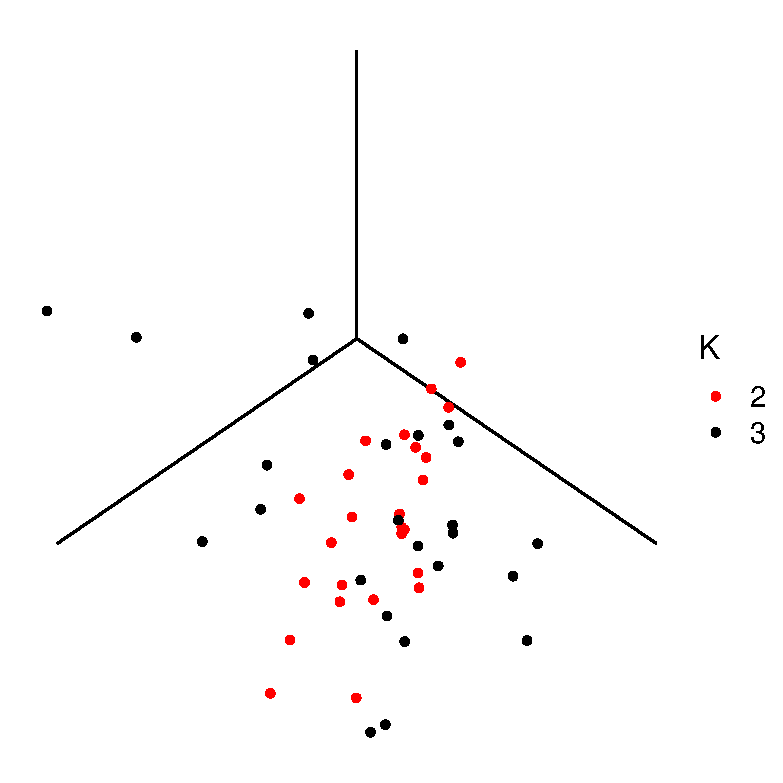
\includegraphics[width=1.0\textwidth]{../images/dim_proj2}}
        \only<4>{\includegraphics[width=1.0\textwidth]{../images/dim_proj1}}
      }
    \end{textblock}
  }
\end{frame}

% JL: Dimensionality
% -------------------------
\begin{frame}{}
  % Content
  \begin{equation*}
    \alert<2>{k} \geq C\frac{\log(\alert<3>{n})}{\alert<4>{\epsilon}^2}
  \end{equation*}
  % Annotation
  \only<2->{%
    \begin{textblock}{4}(+0.5,+0.5)
      {\textblockcolor{}
        $k$ is the projection dimension
      }
    \end{textblock}
  }
  \only<3->{%
    \begin{textblock}{4}(+0.5,+11.0)
      {\textblockcolor{}
        $n$ is the number of observations
      }
    \end{textblock}
  }
  \only<4->{%
    \begin{textblock}{4}(+11.0,+11.0)
      {\textblockcolor{}
        $\epsilon$ is the desired error
      }
    \end{textblock}
  }
  \only<5->{%
    \begin{textblock}{5.0}(+11.0,+0.5)
      {\textblockcolor{}
        Dimensionality is\\
        \emph{curiously absent!}
      }
    \end{textblock}
  }
  \only<6>{%
    \begin{textblock}{4.5}(+5.5,+8.0)
      {\textblockcolor{}
        $k$ is an \emph{intrinsic dimensionality}
      }
    \end{textblock}
  }
\end{frame}

% --------------------------------------------------
%% SEC: Dimension Reduction
% --------------------------------------------------
\framecard{\huge\centering%
  Dimension Reduction
}

% -------------------------
\begin{frame}{Dimension Reduction}
  Idea: Identify low-dimensional structure; \\
  reduce effective dimension

  \bigskip If $\text{Cost} = C^d$, \\
  greatest payoff is reducing $d$
\end{frame}

% -------------------------
\begin{frame}{Dimension Reduction \alert{In UQ}}
  \bigskip \textcolor{palegreen}{J-L showed us \emph{linear} low-dimensional structure} \\
  \textcolor{palered}{J-L does not separate \emph{inputs} and \emph{response}}

  \bigskip We've talked about $\vx$ \\
  What about $f(\vx)$?
\end{frame}

% -------------------------
\begin{frame}{DR Taxonomy}
  \begin{outline}
  \1 Generic-space DR (J-L, PCA, etc.)
    \2 No additional structure on $\R{d}$
  \1 Output-space DR (ROMs, CS, etc.)
    \2 $\R{d}$ is state space, often temporal structure
  \1 \alert<2>{Input-space DR} (CS, ...)
    \2 $\R{d}$ is input space, connected to response
  \end{outline}
\end{frame}

% -------------------------
\begin{frame}{Running Example: Pipe Flow}
  \centering
  \includegraphics[width=0.9\textwidth]{../images/pipe_diagram}

  \begin{textblock}{6.0}(+0.5,+11.0)
    \visible<2>
      {\textblockcolor{}
        qoi: (normalized) pressure loss \\
        inputs: $\rho, u, d, \mu, \epsilon$
      }
  \end{textblock}
\end{frame}

% -------------------------
\begin{frame}{Dimension Reduction: Methods}
  \begin{outline}
    \1 Subset reduction
      \2 Morris screening
      \2 Sobol' indices
    \1 Subspace reduction
      \2 PCA-primer
      \2 Active subspaces
  \end{outline}
\end{frame}

% -------------------------
\begin{frame}{Subset Reduction}
  Suppose $\vx^{\top} = [\vx_A^{\top}, \vx_I^{\top}]$ \\
  What if some variables were \emph{inactive}? E.g.

  \begin{equation*}
    f(\vx_A, \vx_I) = f(\vx_A, \vx'_I),
  \end{equation*}

  \noindent for all $\vx_A$ and $\vx_I \neq \vx'_I$. \\
  Can then \emph{ignore} $\vx_I$.
\end{frame}

% -------------------------
\begin{frame}{Subset Reduction: Methods}
  \begin{outline}
    \1 Morris screening
      \2 \textcolor{palegreen}{Inexpensive}
      \2 \textcolor{palered}{Difficult to interpret}
    \1 Sobol' indices
      \2 \textcolor{palegreen}{Clear interpretation}
      \2 \textcolor{palered}{Can be expensive}
  \end{outline}
\end{frame}

% -------------------------
\begin{frame}{Sobol' Indices}
  Idea: Attribute \emph{variance in output} $f$ \\
  to \emph{different inputs}

  \bigskip E.g.
  \begin{table}
    \centering
    \begin{tabular}{@{}llllll@{}}
     & $\rho$ & $U$ & $d$ & $\mu$ & $\epsilon$\\
    \hline
    $\V[f]$ & 0\% & 0\% & 6\% & 0\% & 94\% \\
    \end{tabular}
  \end{table}

  \visible<2>{\alert{How to \emph{attribute} variance?}}
\end{frame}

% -------------------------
\begin{frame}{Sobol' Formulation}
  Variance decomposition
  \begin{equation*}
    \V[Y] = \E[\V[Y|\mX_{\vu}]] + \V[\E[Y|\mX_{\vu}]]
  \end{equation*}

  Notation: \\
  Ex. $\vu = \{\rho,u,d,\mu\}$ \\
  $-\{\epsilon\} = \{\rho,u,d,\mu\}$
\end{frame}

% -------------------------
\begin{frame}{First-order Index}
   First-order index
  \begin{equation*}
    \underline{\tau}_{\{i\}}^2 = \frac{\alert<3>{\V[\alert<2>{\E[Y|X_i]}]}}{\V[Y]}
  \end{equation*}

  % Annotation
  \visible<2->{Average over \emph{all but} $X_i$\\}
  \visible<3>{Variance due to $X_i$ \emph{alone}}
\end{frame}

% -------------------------
\begin{frame}{Total-order Index}
  Total-order index
  \begin{equation*}
    \overline{\tau}_{\{i\}}^2 = \frac{\alert<3>{\E[\alert<2>{\V[Y|X_{-\{i\}}]}]}}{\V[Y]}
  \end{equation*}

  % Annotation
  \visible<2->{Variance due to \emph{only} $X_i$\\}
  \visible<3>{\emph{Average variance} due to $X_i$ \emph{with interactions}}
\end{frame}

% -------------------------
\begin{frame}{Sobol' Elaboration}
  \begin{equation*} \begin{aligned}
      \text{First} &\leq \text{Total} \\
      0 \leq \underline{\tau}_{\{i\}}^2 &\leq \overline{\tau}_{\{i\}}^2 \leq 1
  \end{aligned} \end{equation*}
\end{frame}

% -------------------------
\begin{frame}{Sobol' Example}
  \begin{equation*} \begin{aligned}
    f(\vx) &= \sin(x_1) + 7\sin^2(x_2) + 0.1 \alert<2->{x_3^4\sin(x_1)} \\
    x_1, x_2, x_3 &\sim U[-\pi, \pi], \\
    \alert<2>{\underline{\tau}_{\{3\}}^2} &= \alert<2>{0\%}, \\
    \alert<3>{\overline{\tau}_{\{3\}}^2} &= \alert<3>{24.4\%}
  \end{aligned} \end{equation*}

  \visible<2->{Input 3 has no main effect}\\
  \visible<3>{\emph{But} input 3 has an interaction}\\
  \footnotetext{\tiny Ishigami \& Homma (1990)}
\end{frame}

% -------------------------
\begin{frame}{But wait...}
  Sobol' indices based on \emph{variance}... \\
  Variance is an \emph{expectation}... \\
  Expectations are \emph{cursed by dimensionality}...

  \bigskip Sobol' is cursed by dimensionality! \\
\end{frame}

% -------------------------
\begin{frame}{Using Sobol'}
  Formulated for analytic models

  \bigskip Surrogate models can extend functionality
\end{frame}

% -------------------------
\begin{frame}{Intrinsic Dimensionality}
  Idea: Find a method whose computational cost scales with \emph{intrinsic
    dimensionality} $k$,\\ \alert{not} dimensionality $d$....
\end{frame}

% -------------------------
\begin{frame}{Subspace Reduction: Methods}
  \begin{outline}
    \1 Principal Component Analysis (PCA)
      \2 Intuition
    \1 Active subspaces
      \2 Application
  \end{outline}
\end{frame}

% -------------------------
\begin{frame}{Principal Component Analysis}
  \huge\underline{Idea:} Find directions that capture variability
\end{frame}

% -------------------------
\framepich{../images/pca1}{}
\framepich{../images/pca2}{}
\framepich{../images/pca3}{
  \begin{textblock}{7}(+9.0,+10.0)
    \visible<2>{
      {\textblockcolor{}
        Direction \alert{from data} \\
        Called \emph{principal component analysis}
      }
    }
  \end{textblock}
}

% -------------------------
\begin{frame}{PCA Formalism}
  Given zero-mean data $\mX\in\R{n\times d}$

  \begin{equation*}
    \mX = \mU\m\Sigma\mV^{\top}
  \end{equation*}

  \noindent with ordered $\sigma_1\geq\dots\geq\sigma_r\geq0$\\
  standard deviations \\

  Select $k \leq d$, project on first $k$ directions, gives new variables
  $\mY\in\R{n\times k}$

  \begin{equation*}
    \mY = \mX\mV_k = \mU\m\Sigma_k
  \end{equation*}

  Often $k$ selected to capture a fraction of the variance
\end{frame}

% -------------------------
\begin{frame}{PCA For Models}
  PCA is for Generic-spaces \\
  How to handle Input-spaces?

  \bigskip Idea: Do a PCA on \emph{gradient data}
\end{frame}

% -------------------------
\framepich{../images/as_contour0}{}
\framepich{../images/as_contour1}{}

% -------------------------
\begin{frame}{Active Subspace}
  \begin{equation*} \begin{aligned}
      \mC &= \E[\nabla_{\vx}f\nabla_{\vx}f^{\top}] \\
          &= \mU\m\Sigma\mV^{\top} \\
          &\approx \frac{1}{n}\sum_{i=1}^n \nabla_{\vx}f_i\nabla_{\vx}f^{\top}_i \\
          &= \hat{\mU}\hat{\m\Sigma}\hat{\mV}^{\top}
  \end{aligned} \end{equation*}

  \footnotetext{\tiny Constantine (2015)}
\end{frame}

% -------------------------
\begin{frame}{AS Selecting $k$}
  Standard arguments bound subspace error based on \emph{eigenvalue gap} $\delta
  = \sigma_{j+1} - \sigma_j$

  \begin{equation*}
    \|\sin(\m\Theta_0)\| \leq \frac{\|\mR\|}{\delta}
  \end{equation*}

  For the pipe flow example
  \begin{table}
    \centering
    \begin{tabular}{@{}ll@{}}
      \hline
      Gap Fraction & Dimension\\
      \hline
      0.9892887 & 1\\
      \hline
      0.0053363 & 2\\
      \hline
      0.0000129 & 3\\
      \hline
      0.0000000 & 4\\
      \hline
    \end{tabular}
  \end{table}

  \footnotetext{\tiny Davis \& Kahan (1970)}
\end{frame}

% -------------------------
\begin{frame}{Using the AS}
  \begin{equation*} \begin{aligned}
      \vx_A &= \mV_A^{\top}\vx \\
      \vx_I &= \mV_I^{\top}\vx
  \end{aligned} \end{equation*}

  \begin{figure}
    \centering
    \includegraphics[width=0.5\textwidth]{../images/as_summary_nat}
  \end{figure}
\end{frame}

% -------------------------
\begin{frame}{But Wait...}
  The active subspace matrix $\mC$ is defined via expectation

  \bigskip It is cursed by dimensionality?
\end{frame}

% -------------------------
\begin{frame}{AS Intrinsic Dimensionality}
  \begin{equation*}
    n \geq \frac{C}{\epsilon^2}\log\left(\frac{4}{p}\text{intdim}(\mC)\right)
  \end{equation*}

  where

  \begin{table}
    \centering
    \begin{tabular}{@{}ll@{}}
      $n$ & Required samples \\
      $\epsilon$ & Desired error tolerance \\
      $p$ & Probability of failure
    \end{tabular}
  \end{table}

  and

  \begin{equation*}
    \text{intdim}(\mC) = \frac{\text{trace}(\mC)}{\|\mC\|_2} \geq 1
  \end{equation*}

  \footnotetext{\tiny Holodnak, Ipsen, and Smith (2018)}
\end{frame}

% -------------------------
\begin{frame}{Intrinsic Dimensionality}
  \huge Where does \emph{intrinsic dimensionality} come from?
\end{frame}

% -------------------------
\begin{frame}{Related Concepts}
  \begin{itemize}
  \item \textbf{Sparsity} -- Compressed sensing
  \item \textbf{Low-rank} -- Linear algebra
  \item \textbf{Dimensionality} -- Dimension reduction
  \visible<2>{\item \textbf{Pi groups} -- Dimensional analysis}
  \end{itemize}
\end{frame}

% -------------------------
\begin{frame}{Dimensional Analysis}
  Buckingham pi

  \begin{equation*} \begin{aligned}
      \pi &= f(\vz) \\
          &= \psi(\pi_1,\dots,\pi_{d-r})
  \end{aligned} \end{equation*}

  where

  \begin{equation}
    \pi_i = \prod_{j=1}^d z_j^{w_{ij}}
  \end{equation}

  \footnotetext{\tiny Buckingham (1914)}
\end{frame}

% -------------------------
\begin{frame}{Dimensional Analysis}
  \alert{Modified}\footnote{del Rosario et al. (2017)} Buckingham pi

  \begin{equation*} \begin{aligned}
      \pi &= f(\vz) \\
          &= \psi'(\mW^{\top}\vx)
  \end{aligned} \end{equation*}

  where $\vx = \log(\vz)$ and

  \begin{equation}
    \mD\mW = 0
  \end{equation}
\end{frame}

% -------------------------
\begin{frame}{DA Example}
  \begin{table}
    \begin{tabular}{@{}lccccc@{}}
      \toprule
      Dimension  & $\rho$ & $u$   & $d$ &  $\mu$ & $\epsilon$\\
      \midrule
      Mass (M)   &   1    &  0    &  0  &    1   &  0 \\
      Length (L) & \mm3   &  1    &  1  &  \mm1  &  1 \\
      Time (T)   &   0    & \mm1  &  0  &  \mm1  &  0 \\
      \bottomrule
      $Re$       &   1    &  1    &  1  &  \mm1  &  0 \\
      $R$        &   0    &  0    & \mm1&    0   &  1
    \end{tabular}
  \end{table}

  \visible{\bigskip Dimensionality $5$\\ Intrinsic dimensionality $2$}
\end{frame}

% -------------------------
\begin{frame}{Pi Subspace}
  Active subspace $\subseteq$ \emph{Pi subspace} $\cR(\mW)$

  \bigskip The pi subspace is \emph{a priori bound on dimensionality}

  \bigskip Intuitive notion of intrinsic dimensionality
\end{frame}

% -------------------------
\begin{frame}{Pi Subspace Example}
  \begin{figure}
    \centering
    \includegraphics[width=0.7\textwidth]{../images/as_summary_pi}
  \end{figure}

  % Annotate
  \begin{textblock}{7}(+6.0,+12.7)
    \visible<2>{%
      \begin{tabular}{@{}llllll@{}}
                & $\rho$ & $u$  & $d$   & $\mu$ & $\epsilon$ \\
        $\vw_1$ & 0.00   & 0.00 & -0.71 & 0.00  & 0.71
      \end{tabular}
    }
  \end{textblock}
\end{frame}

% -------------------------
\framecard{\huge\centering%
  Concluding thoughts
}

% -------------------------
\begin{frame}{The Curse of Dimensionality}
  \begin{itemize}
  \item Is everywhere
  \item Is exponential
  \item Motivates \emph{dimension reduction}
  \end{itemize}
\end{frame}

% -------------------------
\begin{frame}{Dimension Reduction}
  \begin{itemize}
  \item Finds low-dimensional structure
  \item Is tailored to different spaces
  \item Often scales with \emph{intrinsic dimensionality}
  \end{itemize}
\end{frame}

% -------------------------
\begin{frame}{Intrinsic Dimensionality}
  \begin{itemize}
  \item Is problem-dependent
  \item Requires expert judgement
  \item Is waiting to be discovered!
  \end{itemize}

  \bigskip\centering zdr@stanford.edu
\end{frame}

\end{document}
